%%%%%%%%%%%%%%%%%%%%%%%%%%%%%%%%%%%%%%%%%
% University Assignment Title Page 
% LaTeX Template
% Version 1.0 (27/12/12)
%
% This template has been downloaded from:
% http://www.LaTeXTemplates.com
%
% Original author:
% WikiBooks (http://en.wikibooks.org/wiki/LaTeX/Title_Creation)
%
% License:
% CC BY-NC-SA 3.0 (http://creativecommons.org/licenses/by-nc-sa/3.0/)
% 
% Instructions for using this template:
% This title page is capable of being compiled as is. This is not useful for 
% including it in another document. To do this, you have two options: 
%
% 1) Copy/paste everything between \begin{document} and \end{document} 
% starting at \begin{titlepage} and paste this into another LaTeX file where you 
% want your title page.
% OR
% 2) Remove everything outside the \begin{titlepage} and \end{titlepage} and 
% move this file to the same directory as the LaTeX file you wish to add it to. 
% Then add \input{./title_page_1.tex} to your LaTeX file where you want your
% title page.
%
%%%%%%%%%%%%%%%%%%%%%%%%%%%%%%%%%%%%%%%%%
%\title{Title page with logo}
%----------------------------------------------------------------------------------------
%	PACKAGES AND OTHER DOCUMENT CONFIGURATIONS
%----------------------------------------------------------------------------------------

\documentclass[12pt]{article}
\usepackage[english]{babel}
\usepackage[utf8x]{inputenc}
\usepackage{amsmath}
\usepackage{graphicx}
\usepackage[colorinlistoftodos]{todonotes}
\usepackage{subcaption}

\begin{document}

\begin{titlepage}

\newcommand{\HRule}{\rule{\linewidth}{0.5mm}} % Defines a new command for the horizontal lines, change thickness here

\center % Center everything on the page
 
%----------------------------------------------------------------------------------------
%	HEADING SECTIONS
%----------------------------------------------------------------------------------------

% Name of your university/college
\textsc{\LARGE Instituto Superior T\'{e}cnico}\\[1.5cm]
% Major heading such as course name
\textsc{\Large ISR}\\[0.5cm]
% First Minor heading such as course title
\textsc{\large Report}\\[0.25cm]
% Second Minor heading such as course title
\textsc{\small State Of The Art Milestone}\\[0.25cm]

%----------------------------------------------------------------------------------------
%	TITLE SECTION
%----------------------------------------------------------------------------------------

\HRule \\[0.5cm]
{ \large \bfseries A First State Of The Art Essay}\\[0.25cm] % Title of your document
\HRule \\[0.5cm]
 
%----------------------------------------------------------------------------------------
%	AUTHOR SECTION
%----------------------------------------------------------------------------------------

\begin{minipage}{0.4\textwidth}
\begin{flushleft} \large
\emph{Author:}\\
Francisco Maria \textsc{Calisto} % Your name
\end{flushleft}
\end{minipage}
~
\begin{minipage}{0.4\textwidth}
\begin{flushright} \large
\emph{Coordinator:} \\
Professor Jacinto \textsc{Peixoto} % Coordinator's Name
\end{flushright}
~
\begin{flushright} \large
\emph{Co-Coordinator:} \\
Professor Daniel \textsc{Gon\c{c}alves} % Co-Coordinator's Name
\end{flushright}
\end{minipage}\\[2cm]

% If you don't want a supervisor, uncomment the two lines below and remove the section above
%\Large \emph{Author:}\\
%John \textsc{Smith}\\[3cm] % Your name

%----------------------------------------------------------------------------------------
%	DATE SECTION
%----------------------------------------------------------------------------------------

{\large 20/11/2015}\\[2cm] % Date, change the \today to a set date if you want to be precise

%----------------------------------------------------------------------------------------
%	LOGO SECTION
%----------------------------------------------------------------------------------------


\includegraphics{ist-logo.png}\\[0.5cm] % Include a department/university logo - this will require the graphicx package


\includegraphics{isr-logo.png}\\[0.5cm] % Include a department/university logo - this will require the graphicx package
 
%----------------------------------------------------------------------------------------

\vfill % Fill the rest of the page with whitespace

\end{titlepage}

\section{}

%Making a compilation [1] of sketches asked by Professor Jacinto to a better understand of the project as well as to third party who also might need this information, then will outlined the architecture of the issue.
%
%There will be two features, a 1st functionality that will be our focus of the problem and a 2nd feature that will be something developed depending on the course of the project.
%
%\subsection{1st Functionality}
%
%Get the ground-truth [2] (reference measurements), contours, marking the BI-RAD [3] in multi-modality:
%
%% Commands to include a figure:
%\begin{figure}[!hbt]
%\centering
%\includegraphics[width=0.45\textwidth]{isr_1func.png}
%\caption{\label{fig:frog}Ground-Truth}
%\end{figure}
%
%% Commands to include a figure:
%\begin{figure}[!hbt]
%\centering
%\includegraphics[width=0.75\textwidth]{isr_func1_plano3.png}
%\caption{\label{fig:frog}Ground-Truth}
%\end{figure}
%
%\subsection{2nd Functionality}
%
%Proceed to the "follow-up" of the patient, to make the comparison of past data, so we will compare the evolution of the patient thus who we are following by the closer form of injury.
%
%\section{The Meeting}
%\label{sec:examples}
%
%In the presence of Doctor Clara Aleluia the following questions where the feedback has been made:
%
%\subsection{Questions made to the Doctor}
%
%\begin{enumerate}
%  
%  \item Ask if the Doctor just want to have the viewing of 2 breasts or just those that have high probability of occurrence.
%  
%  For this question Doctor said that usually the viewing is done observing both breasts at the same time to compare the symmetries of the images, for this same symmetry is the first act in checking something wrong in the breast.
%  
%  \item Understand the meaning of traits for the Doctor.
%  
%  For the Doctor this feature will serve as we have for example a situation where we go as the points are taken there will be lines that connect them to each other and this is the defining traits. It is important to have an undo feature and undo the points made (redo and undo) also giving the possibility to change a given point (example: alter the 3rd point). For the Doctor it is needed about 10 points on an average estimated by itself and informally.
%  
%  \item Understand what are calcifications and aggregate of a breast as clinical terms.
%  
%  In this part I was pretty savvy and demonstrate step by step the means by using images:
%  
%% Commands to include a figure:
%\begin{figure}[!hbt]
%\centering
%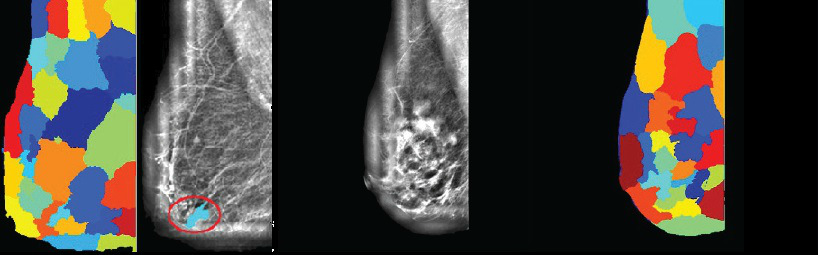
\includegraphics[width=0.75\textwidth]{breast_aggregates.png}
%\caption{\label{fig:frog}Breast Aggregates}
%\end{figure}
%
%% Commands to include a figure:
%\begin{figure}[!hbt]
%\centering
%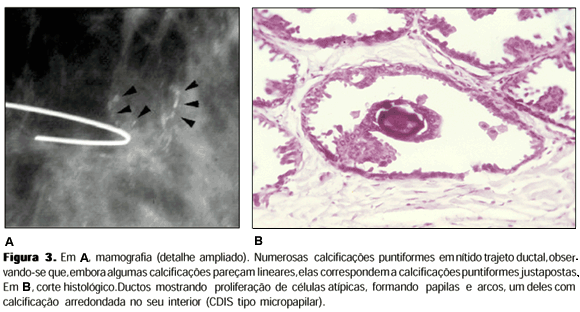
\includegraphics[width=0.75\textwidth]{breast_calcifications.png}
%\caption{\label{fig:frog}Breast Calcifications}
%\end{figure}
%  
%  \item What are the Doctor preferences and medical routines for interaction with the machine?
%  
%  Here it was also observed with the Doctor an attention need for the interaction with the machine and it was observed a much greater choice thereof to handle a computer mouse.
%  
%  \item Understand if the doctor wants to write down all the slices, or otherwise, which slice you want to note?
%  
%  To this question the Doctor said that would depend on where the changes are sweeping the slices and then selecting the slice to note.
%  
%  \item Is it important to have always visible state of the system, even if it means losing screen space?
%  
%   In this case, we have to be careful about the relevance of this question in given circumstances, it is important to tell the interface image where you are watching over the others and whether it is right breast or the left breast. The rest of the information it seemed negligible and not useful, being most important for the Doctor gain screen space face to have less visible information system.
%  
%  \item Can we have access to the software currently being used?
%  
%  The software is all available online, with a range of software for this type of clinical evaluations is called a PACS [4]. There is enough information about this range of software in Google Scholar [5] as shown as well as some papers [6]. The software used in Hospital Amadora Sintra Carestream Vue PACS [7] is nevertheless also have the OsiriX [8].
%
%\end{enumerate}

%\subsection{Comments}
%
%There was indeed a greater importance in the use and iteration mouse over the keyboard by the Doctor. Where the right side of the mouse is not used at the moment by the Software that the Doctor uses and has the potential to be used in ours.
%
%It is important to have text notations and notations using symbols, such as arrows and other symbols to write down calcifications, masses and corresponding Bi-RADS.
%
%There are no visible calcifications in the MRI and is usually verified later in the visualisation process.
%
%There are masses in Mamo, Echo and MRI.
%
%It must have a labelling field on the images.
%
%The 2nd functionality, the "follow-up" functionality primarily has the objective of information selection, as well as display information (VI), which in general controls are done a minimum of 6 months having 1 inspections at 1 year and evolutions They are usually seen in space five years.
%
%\section{Project Management}
%
%It is essential that the Coordinator proceed to a meeting with the Co-Coordinator, in this phase, to define what the goals, objectives and methodologies to address in this project, because only from here I can move forward. Ideally will be Professor Jacinto talk with Professor Daniel and after that arrange a meeting three to better discuss what they said. I would like therefore to be aware of the meeting between the two.
%
%Regarding methodologies have been analysing calmly a few ways to address developments in this order. There are basic and general ways of treating these projects such as the DSR [9] technique for iterating projects:
%
%% Commands to include a figure:
%\begin{figure}[!hbt]
%\centering
%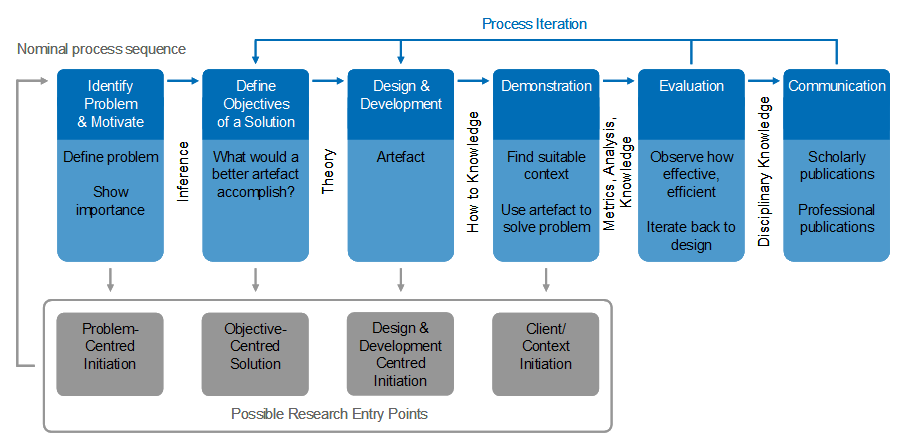
\includegraphics[width=0.75\textwidth]{diss_goebel_2.png}
%\caption{\label{fig:frog}DSR}
%\end{figure}
%
%In this case we are talking not of Interface but the whole development of the Master Project, which for is no longer our main concern.
%
%In terms of interface we have two methodologies that I consider they are the only ones in the academic course attended:
%
%% Commands to include a figure:
%\begin{figure}[!hbt]
%\centering
%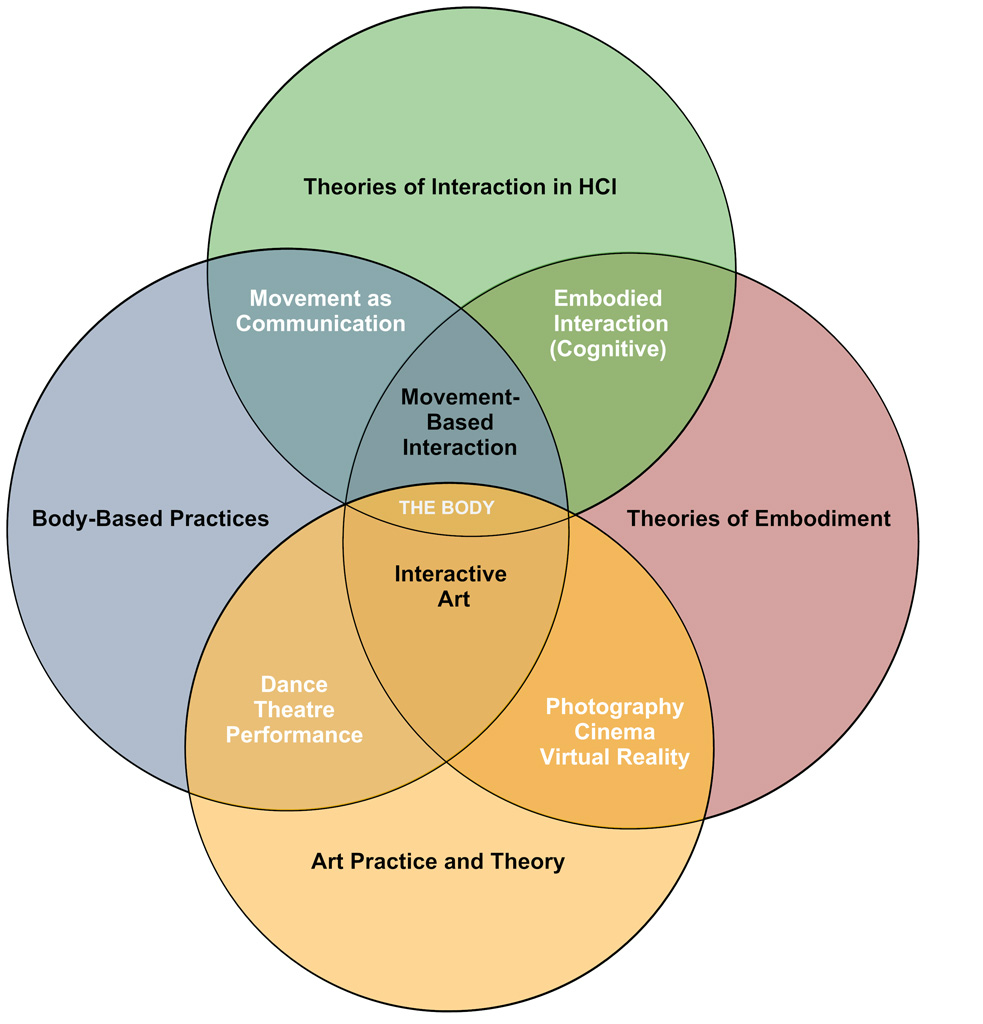
\includegraphics[width=0.50\textwidth]{ven-diagram.png}
%\caption{\label{fig:frog}HCI Methodologies}
%\end{figure}
%
%- Human-Computer Interaction Methodologies [10] (Figure 6);
%
%% Commands to include a figure:
%\begin{figure}[!hbt]
%\centering
%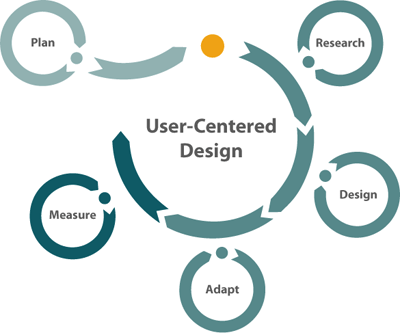
\includegraphics[width=0.50\textwidth]{ucd_new.png}
%\caption{\label{fig:frog}UCD Methodologies}
%\end{figure}
%
%- User-Centered Design Methodologies [11] (Figure 7);
%
%\clearpage

%\begin{thebibliography}{}
%\bibitem{GitHub} Project and Clinical Environment Presentation (PCEP) Report Repository, \emph{github.com}[online], (https://github.com/FMCalisto/master-project/tree/master/reports/hospital-meetings/report\_1).
%\bibitem{Wikipedia} Ground-truth, \emph{wikipedia.org}[online], (https://en.wikipedia.org/wiki/Ground\_truth).
%\bibitem{Wikipedia} BI-RADS, \emph{wikipedia.org}[online], (https://en.wikipedia.org/wiki/BI-RADS).
%\bibitem{Wikipedia} Picture archiving and communication system, \emph{wikipedia.org}[online], (https://en.wikipedia.org/wiki/Picture\_archiving\_and\_communication\_system).
%\bibitem{Google} PACS Picture Archiving and Communication System, \emph{scholar.google.com}[online], (http://tinyurl.com/pfoqfvt).
%\bibitem{Wikipedia} PACS - Picture Archiving and Communication System, Maximilian Hecht, \emph{cg.tuwien.ac.at}[online], Vienna University of Technology, University of Paderborn, (https://www.cg.tuwien.ac.at/courses/Seminar/WS2009/PACS.pdf).
%\bibitem{CARESTREAM} CARESTREAM Vue PACS, \emph{carestream.com}[online], (http://www.carestream.com/vue-pacs.html).
%\bibitem{Osirix} Osirix, \emph{osirix-viewer.com}[online], (http://www.osirix-viewer.com/).
%\bibitem{Wikipedia} Design science research, \emph{wikipedia.org}[online], (https://en.wikipedia.org/wiki/Design\_science\_research).
%\bibitem{Wikipedia} Human–computer interactio, Methodologies, \emph{wikipedia.org}[online], (https://en.wikipedia.org/wiki/Human\%E2\%80\%93computer\_interaction\#Methodologies).
%\bibitem{Wikipedia} User-centered design, \emph{wikipedia.org}[online], (https://en.wikipedia.org/wiki/User-centered\_design).
%\end{thebibliography}


%\fi %comment me out

\end{document}
